\section{Average Lateral Error (ALE) (reported in the paper)}
Average lateral error is the 2-norm of the perpendicular distance $\tilde{y}$
to the robot heading direction averaged over entire time $T$ of the trajectory. 
\begin{figure*}[h]
  \begin{minipage}{0.5\textwidth}
  \begin{equation} \label{eq:ale}
    \text{ALE} = \sqrt{\frac{||\tilde{y}||_2^2}{T}} 
    = \sqrt{\frac{\int_{0}^{T} \tilde{y}(t)^2 \,dt}{T}}
  \end{equation}
  \end{minipage}
  \hfill
  \begin{minipage}{0.49\textwidth}
    \vspace*{0.06in}
    \centering
    \begin{tikzpicture}[inner sep=0pt,outer sep=0pt]
	  \node[anchor=south west] (pop) at (0in, 0in)
      {{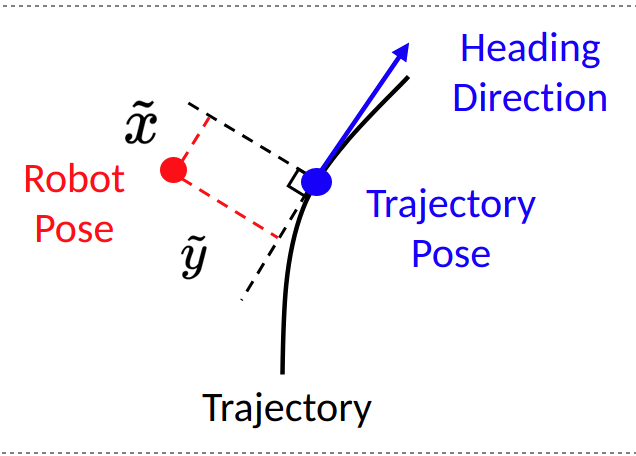
\includegraphics[height=0.9in,clip=true,trim=0.25in 0.1in
      0.25in 0.25in]{figs/ale_fig.png}}};
    \end{tikzpicture}
    \vspace*{-7pt}
    \caption{Lateral Error $\tilde{y}$ \label{fig:ale}}
  \end{minipage}  
  \vspace*{-1.5em}
\end{figure*}

\subsection{Short Distance Simulation Outcomes}
\vspace*{-0.5em}
\begin{figure*}[h]
\begin{minipage}[t]{\textwidth}
\centering
%\vspace*{-1.45in}
\captionof{table}{ Short distance simulation ALE outcomes.\label{tab:shortALE}}
\vspace*{-0.5em}
\begin{tikzpicture}[inner sep=0pt,outer sep=0pt,scale=1, every node/.style={scale=0.8}]
    % sim ALE
	\node[anchor=north west] (sim_ale) at (0, 0pt)
    {
    \setlength{\tabcolsep}{4pt}
    \begin{tabular}{|c||c|ccc|}
    \hline 
    \textbf{Seq.} & PO & SLAM & TS & VS+ \\ 
    \hline 
%       &       &       & SLAM  & $\neg$SLAM \\
    SS  & 0.70  & 0.84  & 0.88  & x \\ 
    SWT & 0.71  & 1.35  & 1.23  & x \\ 
    SST & 0.55  & 1.64  & 0.82  & x \\ 
    STS & 0.86  & 1.68  & 0.91  & x \\ 
    STT & 0.75  & 1.21  & 0.96  & x \\ 
    \hline 
    \textbf{Avg.} & 0.71 & 1.34 & \textbf{0.96} & x \\ 
    %\textbf{Std. ATE} & 0.0000 & 0.0000 & 0.0000 \\
%    & \textcolor{white}{$v,\omega$} & & & \\
    \hline 
    \end{tabular}
    };
    
    \node[anchor=south, text width=5cm, text centered] (sim_ale_cap) 
    at ($(sim_ale.north) + (0pt, 2pt)$)
    {\normalsize \textbf{(a)} Sim {ALE} (cm)};
      
    % p-values
    \node[anchor=west] (sim_ale_p) at ($(sim_ale.east) + (5pt, 0)$)
    {
    \setlength{\tabcolsep}{5pt}
    \begin{tabular}{|l||c|}
    \hline 
    \textbf{PO} vs \textbf{SLAM} & \textless 1e-5 \\ 
    \hline 
    \textbf{PO} vs \textbf{TS} & 2e-3 \\ 
    \hline
    \textbf{SLAM} vs \textbf{TS} & 8.4e-4 \\ 
    \hline 
    \end{tabular}
    };
    
	\node[anchor=south, text width=5cm, text centered] (sim_ale_p_cap) 
    at ($(sim_ale_p.north) + (0pt, 2pt)$)
    {\normalsize \textbf{(b)} p-values of \\ pairwise comparisons};        

\end{tikzpicture}
\end{minipage}
\vspace*{-1.5em}
\end{figure*}

%\pagebreak
\subsection{Long Distance Simulation Outcomes}
\vspace*{-0.5em}
\begin{figure*}[h]
\begin{minipage}[t]{\textwidth}
\centering
%\vspace*{-1.45in}
\captionof{table}{ Long distance simulation ALE outcomes.\label{tab:longALE}}
\vspace*{-0.5em}
\begin{tikzpicture}[inner sep=0pt,outer sep=0pt,scale=1, every node/.style={scale=0.8}]
    % sim ALE
	\node[anchor=north west] (sim_ale) at (0, 0pt)
    {
    \setlength{\tabcolsep}{4pt}
    \begin{tabular}{|c||c|cc|c|}
    \hline 
    \textbf{Seq.} & PO & SLAM & TS & TS+PO \\ 
    \hline 
%      & \textcolor{white}{$v,\omega$} & & \\
    LRU & 0.53  & 3.88  & 4.00  & 1.47 \\ 
    LLU & 0.86  & 8.21  & 5.18  & 1.61 \\ 
    LST & 1.13  & 5.03  & 3.00  & 2.03 \\ 
    LZZ & 1.06  & 7.54  & 5.90  & 5.04 \\ 
    \hline 
    \textbf{Avg.} & 0.90 & 6.17 & \textbf{4.52} & 2.54 \\
    \hline 
    \end{tabular}
    };
    
    \node[anchor=south, text width=5cm, text centered] (sim_ale_cap) 
    at ($(sim_ale.north) + (0pt, 2pt)$)
    {\normalsize \textbf{(a)} Sim {ALE} (cm)};
      
    % p-values
    \node[anchor=west] (sim_ale_p) at ($(sim_ale.east) + (5pt, 0)$)
    {
    \setlength{\tabcolsep}{5pt}
    \begin{tabular}{|l||c|}
    \hline 
    \textbf{PO} vs \textbf{SLAM} & \textless 1e-5 \\ 
    \hline 
    \textbf{PO} vs \textbf{TS} & \textless 1e-5 \\ 
    \hline
    \textbf{PO} vs \textbf{TS+PO} & 5e-3 \\ 
    \hline 
    \textbf{SLAM} vs \textbf{TS} & 1.4e-3 \\ 
    \hline 
    \textbf{SLAM} vs \textbf{TS+PO} & \textless 1e-5 \\ 
    \hline 
    \textbf{TS} vs \textbf{TS+PO} & 2.1e-3 \\ 
    \hline 
    \end{tabular}
    };
    
	\node[anchor=south, text width=5cm, text centered] (sim_ale_p_cap) 
    at ($(sim_ale_p.north) + (0pt, 2pt)$)
    {\normalsize \textbf{(b)} p-values of \\ pairwise comparisons};       

\end{tikzpicture}
\end{minipage}
  \vspace*{-1.5em}
\end{figure*}
